% Scatter plot showing 60 evaluations (12 conditions × 5 seeds)
% All Faith.-NLI points sit at y=0.84, all EM-F1 points at y=0.3979
% Horizontal jitter ±0.10 is hard-coded per seed offset
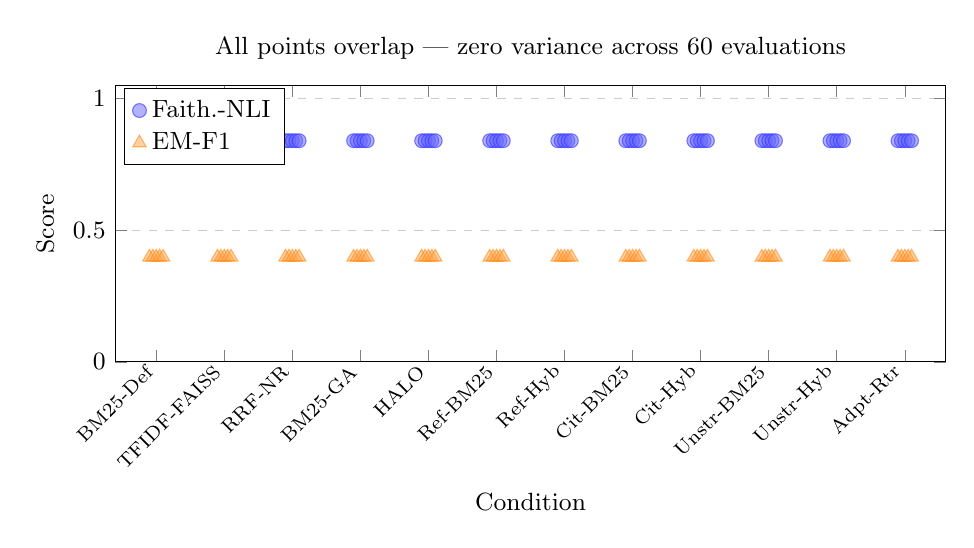
\begin{tikzpicture}
\begin{axis}[
  compat=1.18,
  width=\textwidth,
  height=0.42\textwidth,
  xmin=-0.6, xmax=11.6,
  ymin=0, ymax=1.05,
  ylabel={Score},
  ylabel style={font=\small},
  xlabel={Condition},
  xlabel style={font=\small},
  xtick={0,1,2,3,4,5,6,7,8,9,10,11},
  xticklabels={BM25-Def, TFIDF-FAISS, RRF-NR, BM25-GA, HALO,
               Ref-BM25, Ref-Hyb, Cit-BM25, Cit-Hyb,
               Unstr-BM25, Unstr-Hyb, Adpt-Rtr},
  x tick label style={font=\scriptsize, rotate=45, anchor=east},
  y tick label style={font=\small},
  legend style={at={(0.01,0.99)}, anchor=north west, font=\small},
  legend cell align=left,
  ymajorgrids=true,
  grid style={dashed, gray!40},
  title={\small All points overlap --- zero variance across 60 evaluations},
  title style={font=\small},
]

% Faith.-NLI: 5 seeds per condition, jitter offsets: -0.10,-0.05,0,+0.05,+0.10
\addplot[only marks, mark=*, mark options={fill=blue!60, draw=blue!80,
         fill opacity=0.5, draw opacity=0.6}, mark size=2.5pt]
  coordinates {
    % cond 0
    (-0.10,0.84)(-0.05,0.84)(0,0.84)(0.05,0.84)(0.10,0.84)
    % cond 1
    (0.90,0.84)(0.95,0.84)(1,0.84)(1.05,0.84)(1.10,0.84)
    % cond 2
    (1.90,0.84)(1.95,0.84)(2,0.84)(2.05,0.84)(2.10,0.84)
    % cond 3
    (2.90,0.84)(2.95,0.84)(3,0.84)(3.05,0.84)(3.10,0.84)
    % cond 4
    (3.90,0.84)(3.95,0.84)(4,0.84)(4.05,0.84)(4.10,0.84)
    % cond 5
    (4.90,0.84)(4.95,0.84)(5,0.84)(5.05,0.84)(5.10,0.84)
    % cond 6
    (5.90,0.84)(5.95,0.84)(6,0.84)(6.05,0.84)(6.10,0.84)
    % cond 7
    (6.90,0.84)(6.95,0.84)(7,0.84)(7.05,0.84)(7.10,0.84)
    % cond 8
    (7.90,0.84)(7.95,0.84)(8,0.84)(8.05,0.84)(8.10,0.84)
    % cond 9
    (8.90,0.84)(8.95,0.84)(9,0.84)(9.05,0.84)(9.10,0.84)
    % cond 10
    (9.90,0.84)(9.95,0.84)(10,0.84)(10.05,0.84)(10.10,0.84)
    % cond 11
    (10.90,0.84)(10.95,0.84)(11,0.84)(11.05,0.84)(11.10,0.84)
  };
\addlegendentry{Faith.-NLI}

% EM-F1: same jitter pattern at y=0.3979
\addplot[only marks, mark=triangle*, mark options={fill=orange!70, draw=orange!90,
         fill opacity=0.5, draw opacity=0.6}, mark size=2.8pt]
  coordinates {
    % cond 0
    (-0.10,0.3979)(-0.05,0.3979)(0,0.3979)(0.05,0.3979)(0.10,0.3979)
    % cond 1
    (0.90,0.3979)(0.95,0.3979)(1,0.3979)(1.05,0.3979)(1.10,0.3979)
    % cond 2
    (1.90,0.3979)(1.95,0.3979)(2,0.3979)(2.05,0.3979)(2.10,0.3979)
    % cond 3
    (2.90,0.3979)(2.95,0.3979)(3,0.3979)(3.05,0.3979)(3.10,0.3979)
    % cond 4
    (3.90,0.3979)(3.95,0.3979)(4,0.3979)(4.05,0.3979)(4.10,0.3979)
    % cond 5
    (4.90,0.3979)(4.95,0.3979)(5,0.3979)(5.05,0.3979)(5.10,0.3979)
    % cond 6
    (5.90,0.3979)(5.95,0.3979)(6,0.3979)(6.05,0.3979)(6.10,0.3979)
    % cond 7
    (6.90,0.3979)(6.95,0.3979)(7,0.3979)(7.05,0.3979)(7.10,0.3979)
    % cond 8
    (7.90,0.3979)(7.95,0.3979)(8,0.3979)(8.05,0.3979)(8.10,0.3979)
    % cond 9
    (8.90,0.3979)(8.95,0.3979)(9,0.3979)(9.05,0.3979)(9.10,0.3979)
    % cond 10
    (9.90,0.3979)(9.95,0.3979)(10,0.3979)(10.05,0.3979)(10.10,0.3979)
    % cond 11
    (10.90,0.3979)(10.95,0.3979)(11,0.3979)(11.05,0.3979)(11.10,0.3979)
  };
\addlegendentry{EM-F1}

\end{axis}
\end{tikzpicture}
